\section{Packages}

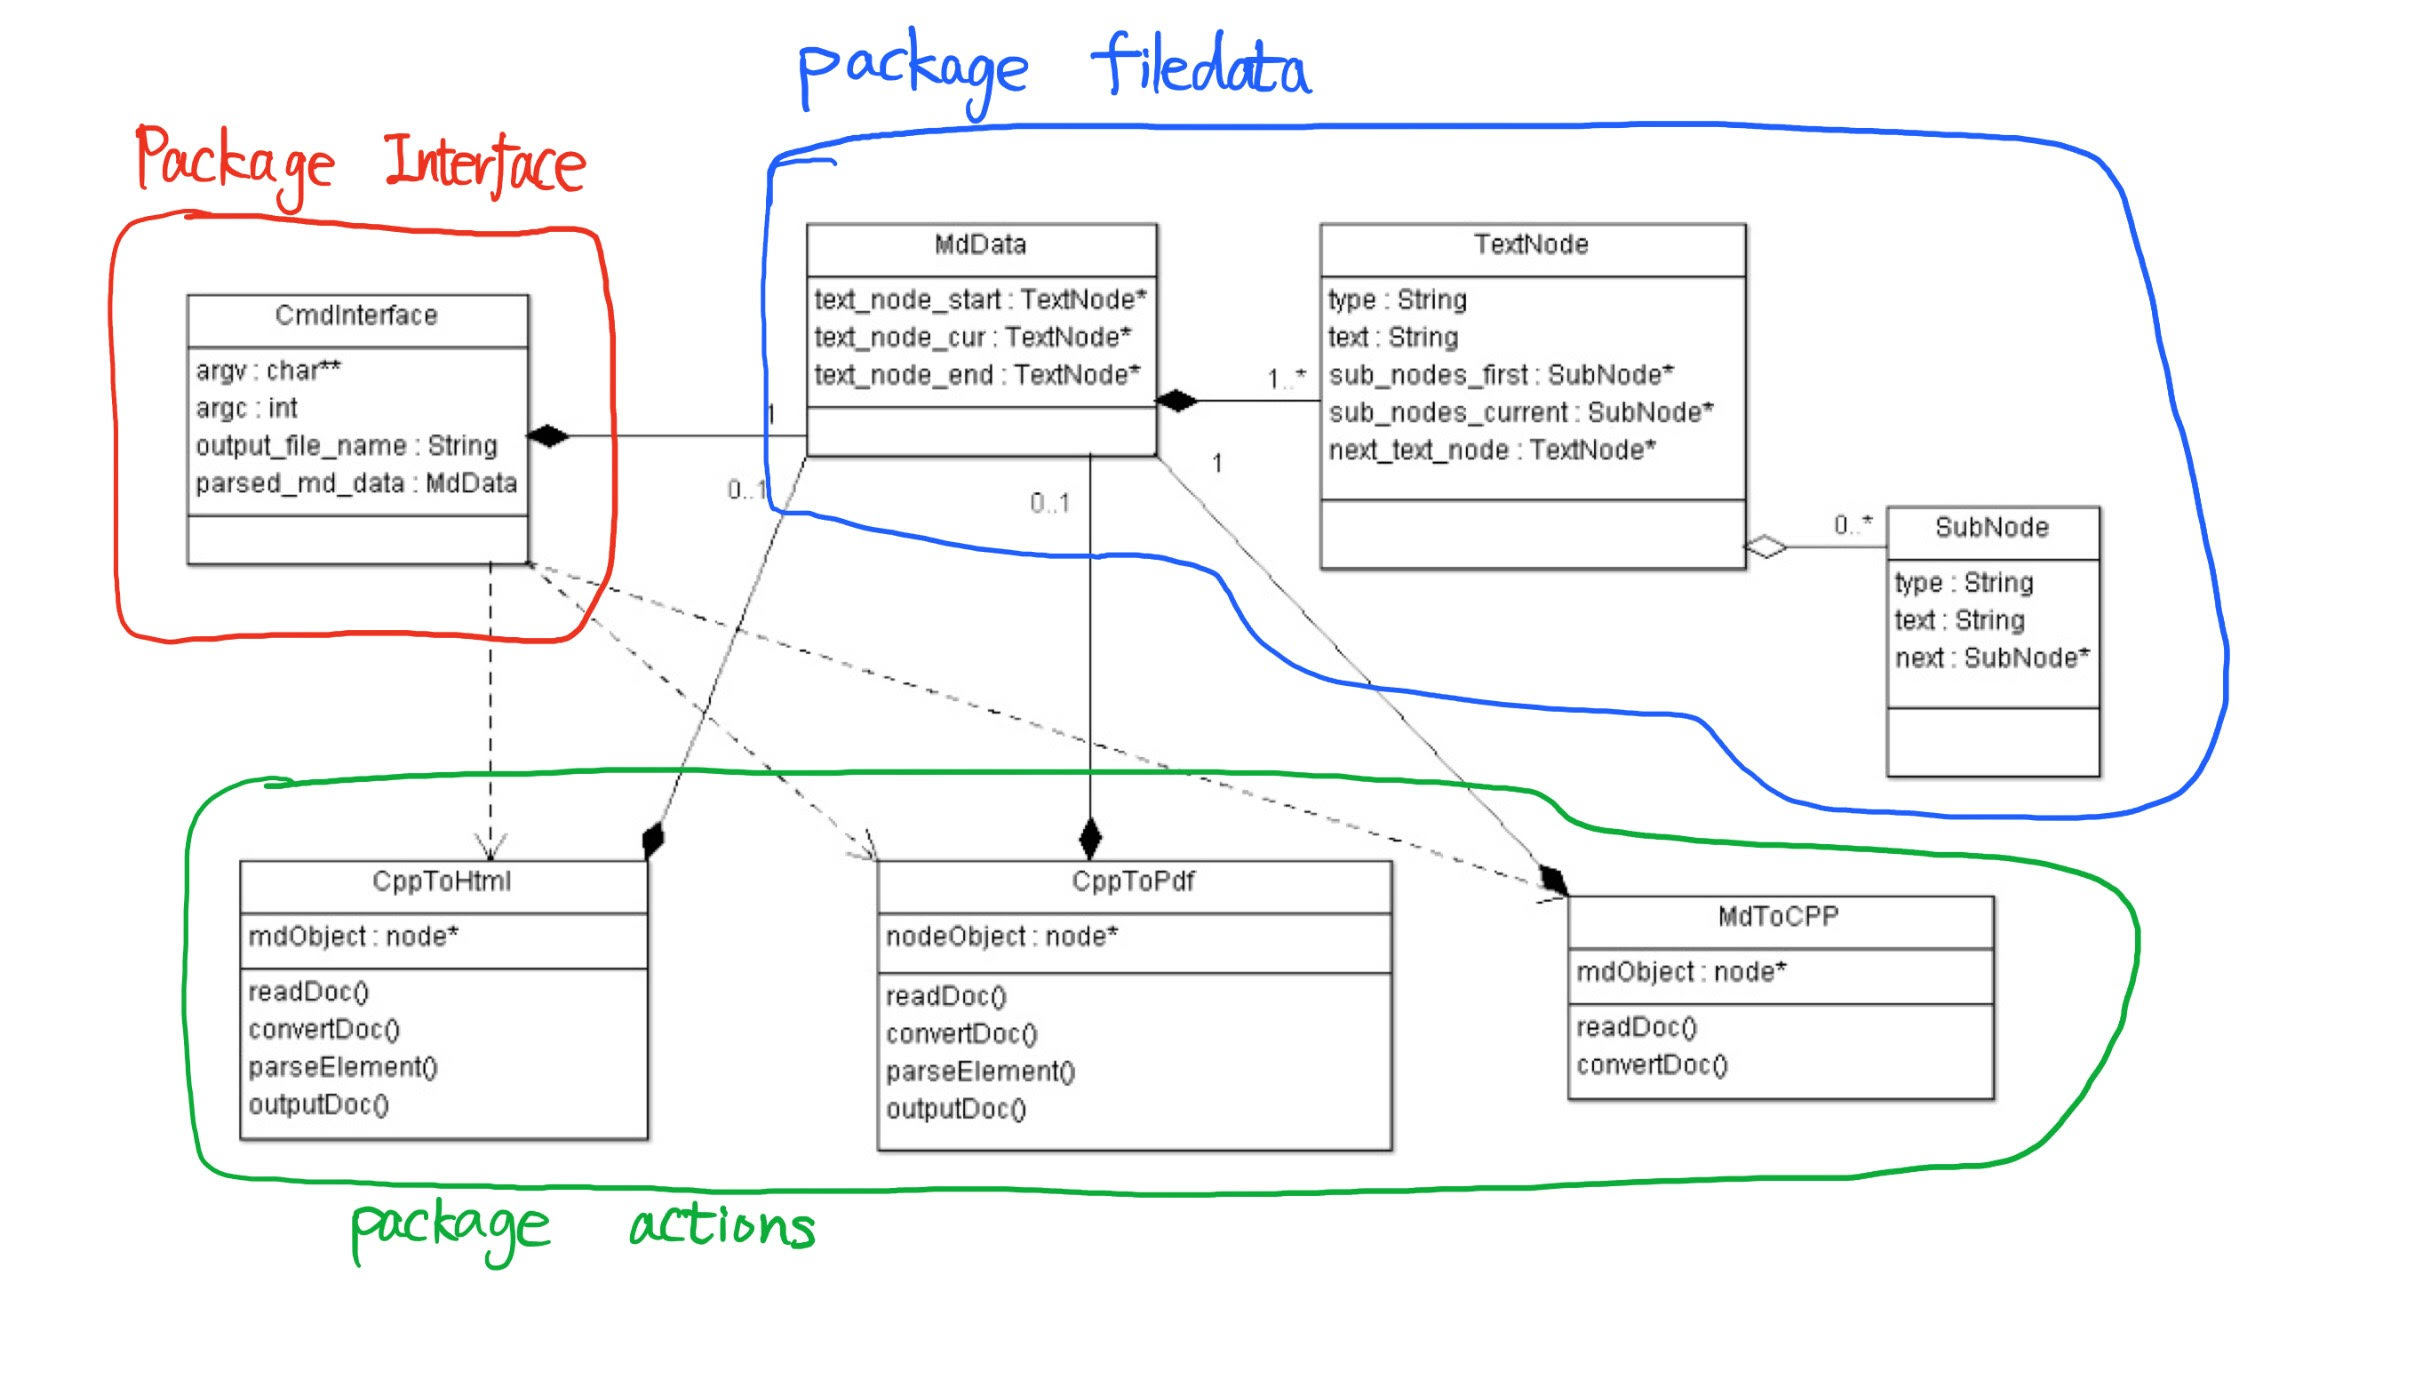
\includegraphics[width=500pt]{images/Packages.png}
\textbf{Packages:}
\begin{itemize}
\item Interface: Takes in command line arguments and decides what to do.
\item filedata:  Read and return markdown data.
\item Actions:   Actions will be selected by user, then they will convert and output the corresponding data or file with requirements
\end{itemize}
\textbf{Low coupling and high cohesion:}
\begin{itemize}
\item Maintainability: packages are distinguished clearly from their functions, which makes the program clear for tracking bugs and maintenace within a single module
\item Understandability: related classes and functions are contained in a single module, this make the program's codes easy to read.
\end{itemize}
